\chapter{心脏与循环}\label{ch:g7:heart-and-circulation}

\Cref{ch:g4:heart-and-blood}已介绍了泵及其
往返输送的功能；此后\omterm{prop:g4:journey-of-food:absorb}{血液}又承担了
新的职责——在\omterm{prop:g7:digestion-and-nutrients:absorption}{绒毛}处接收\omterm{def:g7:digestion-and-nutrients:families}{营养物质}
（\cref{prop:g7:digestion-and-nutrients:absorption}），在\omterm{def:g7:lungs-and-gas-exchange:alveoli}{肺泡}处
运送\omterm{def:g7:what-is-respiration:respiration}{氧气}
（\cref{prop:g7:lungs-and-gas-exchange:numbers}），在每块工作
的\omterm{def:g3:bones-and-muscles:muscle}{肌肉}处都要“结账”（\cref{prop:g7:organs-at-work:bill}）。
现在来认真绘制这张“道路网”：\omterm{def:g4:heart-and-blood:heart}{心脏}的四个
腔室、两条循环路线和三类\omterm{def:g4:heart-and-blood:vessels}{血管}。

\section{心脏的四个腔室}

\begin{definition}[心房与心室]\label{def:g7:heart-and-circulation:rooms}
\omterm{def:g4:heart-and-blood:heart}{心脏}的左右两侧（\cref{def:g4:heart-and-blood:heart}）
各含两个腔室：上方的
\emph{心房}\index{心房}，负责接收流入的\omterm{prop:g4:journey-of-food:absorb}{血液}，
下方的\emph{心室}\index{心室}（厚壁的
泵血腔室）负责把\omterm{prop:g4:journey-of-food:absorb}{血液}泵出。
在腔室之间及其出入口处，设有\emph{瓣膜}\index{瓣膜（心脏）}——
单向的“门”——每次血流涌过后随即关闭；
两次闭合的声响正是听诊器（或
贴在胸口的耳朵）所听到的“咚—哒”声。
\end{definition}

\begin{proposition}[一次搏动，依次进行]\label{prop:g7:heart-and-circulation:beat}
每次搏动，左右两侧同时按相同顺序进行：
\omterm{def:g7:heart-and-circulation:rooms}{心房}收缩，为\omterm{def:g7:heart-and-circulation:rooms}{心室}补充\omterm{prop:g4:journey-of-food:absorb}{血液}；\omterm{def:g7:heart-and-circulation:rooms}{心室}
收缩，将\omterm{prop:g4:journey-of-food:absorb}{血液}泵出——右侧
泵向肺，左侧泵向全身——与此同时，
入口处的\omterm{def:g7:heart-and-circulation:rooms}{瓣膜}关闭（咚）；\omterm{def:g7:heart-and-circulation:rooms}{心室}舒张，出口
处的\omterm{def:g7:heart-and-circulation:rooms}{瓣膜}关闭（哒），腔室重新充盈。随后循环往复，
每天 $100000$ 次
（\cref{rem:g4:heart-and-blood:rest}）。
\end{proposition}
\admitted

\section{两条循环，三类血管}

\begin{definition}[双循环]\label{def:g7:heart-and-circulation:double}
\omterm{prop:g4:journey-of-food:absorb}{血液}的道路网由经过同一台泵的两条环路构成
（\cref{def:g4:heart-and-blood:heart}中的左右两侧，
此处以循环路线的形式呈现）：
\begin{itemize}
  \item \emph{肺循环}：右\omterm{def:g7:heart-and-circulation:rooms}{心室}
        $\rightarrow$ 肺（摄入\omterm{def:g7:what-is-respiration:respiration}{氧气}、排出
        \omterm{def:g7:what-is-respiration:respiration}{二氧化碳}）$\rightarrow$ 左\omterm{def:g7:heart-and-circulation:rooms}{心房}；
  \item \emph{体循环}：左\omterm{def:g7:heart-and-circulation:rooms}{心室}
        $\rightarrow$ 全身（输送、
        回收）$\rightarrow$ 右\omterm{def:g7:heart-and-circulation:rooms}{心房}。
\end{itemize}
每一滴血都交替经过两条循环：肺、体、肺、体——
这正是左\omterm{def:g7:heart-and-circulation:rooms}{心室}，要推动远为庞大的
体循环，因此成为\omterm{def:g4:heart-and-blood:heart}{心脏}中室壁最厚的
腔室。
\end{definition}

\begin{definition}[动脉、毛细血管、静脉]\label{def:g7:heart-and-circulation:vessels}
每条循环都由三类\omterm{def:g4:heart-and-blood:vessels}{血管}构成
（\cref{def:g4:heart-and-blood:vessels}，此处给出正式名称）：
\begin{itemize}
  \item \emph{动脉}\index{动脉}：管壁厚、
        有弹性，将\omterm{prop:g4:journey-of-food:absorb}{血液}\emph{远离}
        \omterm{def:g4:heart-and-blood:heart}{心脏}，承受较高压强——\omterm{prop:g4:heart-and-blood:pulse}{脉搏}
        （\cref{prop:g4:heart-and-blood:pulse}）即是动脉
        在每次血流涌入时的扩张；
  \item \emph{毛细血管}\index{毛细血管}：
        遍布各器官的发丝般细\omterm{def:g4:heart-and-blood:vessels}{血管}——
        管壁只有一个\omterm{def:g5:first-look-at-cells:cell}{细胞}厚，是\emph{所有}
        物质交换发生的场所：\omterm{def:g7:lungs-and-gas-exchange:alveoli}{肺泡}、\omterm{prop:g7:digestion-and-nutrients:absorption}{绒毛}、\omterm{def:g3:bones-and-muscles:muscle}{肌肉}、\omterm{def:g1:the-five-senses:sense}{皮肤}；
  \item \emph{静脉}\index{静脉}：管腔宽，管壁较薄，
        将\omterm{prop:g4:journey-of-food:absorb}{血液}\emph{送回}\omterm{def:g4:heart-and-blood:heart}{心脏}，压强较低，
        自身也有单向\omterm{def:g7:heart-and-circulation:rooms}{瓣膜}——
        蓝色线条，见
        \cref{rem:g4:heart-and-blood:see}。
\end{itemize}
\end{definition}

\begin{omfigure}
\begin{tikzpicture}[scale=0.9]
  % heart center: four rooms
  \draw[thick] (3.8,2.1) rectangle (7.0,3.9);
  \draw[thick] (5.4,2.1) -- (5.4,3.9);
  \draw[thick] (3.8,3.0) -- (7.0,3.0);
  \node[font=\footnotesize, align=center] at (4.6,3.45)
    {右 \\心房};
  \node[font=\footnotesize, align=center] at (6.2,3.45)
    {左 \\心房};
  \node[font=\footnotesize, align=center] at (4.6,2.55)
    {右 \\心室};
  \node[font=\footnotesize, align=center] at (6.2,2.55)
    {左 \\心室};
  % lungs above
  \draw[thick, fill=omDef!8] (4.5,5.2) ellipse (0.75 and 0.6);
  \draw[thick, fill=omDef!8] (6.3,5.2) ellipse (0.75 and 0.6);
  \node[font=\footnotesize] at (5.4,5.95) {肺};
  % body below
  \draw[thick, fill=omProp!8, rounded corners=6pt]
    (3.9,-0.7) rectangle (6.9,0.5);
  \node[font=\footnotesize] at (5.4,-0.1) {全身};
  % lung circuit arrows
  \draw[->, very thick, omDef] (4.9,3.9) .. controls (4.6,4.4)
    .. (4.5,4.6);
  \draw[->, very thick, omThm] (6.3,4.6) .. controls (6.2,4.35)
    .. (5.95,3.92);
  \node[font=\footnotesize, omDef, left] at (4.35,4.45)
    {装载氧气};
  % body circuit arrows
  \draw[->, very thick, omThm] (5.95,2.1) .. controls (6.3,1.3)
    .. (6.2,0.52);
  \draw[->, very thick, omDef] (4.6,0.52) .. controls (4.5,1.3)
    .. (4.9,2.08);
  \node[font=\footnotesize, omThm, right] at (6.45,1.3)
    {输出};
  \node[font=\footnotesize, omDef, left] at (4.3,1.3)
    {回流};
\end{tikzpicture}

{\small 双循环：右侧将\omterm{prop:g4:journey-of-food:absorb}{血液}送往肺，再回到左侧；
左侧将\omterm{prop:g4:journey-of-food:absorb}{血液}送往全身，再回到右侧。
红色箭头表示富含\omterm{def:g7:what-is-respiration:respiration}{氧气}的段落，
蓝色表示回流的段落。}
\end{omfigure}

\begin{example}[一滴血的完整旅程]\label{ex:g7:heart-and-circulation:tour}
\Cref{ex:g4:heart-and-blood:round}中的输送路线，
并使用图中的名称：右\omterm{def:g7:heart-and-circulation:rooms}{心室}——肺\omterm{def:g7:heart-and-circulation:vessels}{毛细血管}
（在\omterm{def:g7:lungs-and-gas-exchange:alveoli}{肺泡}处载上\omterm{def:g7:what-is-respiration:respiration}{氧气}，呈鲜红色）——左\omterm{def:g7:heart-and-circulation:rooms}{心房}，
左\omterm{def:g7:heart-and-circulation:rooms}{心室}——\omterm{def:g7:heart-and-circulation:vessels}{动脉}——大腿\omterm{def:g3:bones-and-muscles:muscle}{肌肉}的\omterm{def:g7:heart-and-circulation:vessels}{毛细血管}
（释放\omterm{def:g7:what-is-respiration:respiration}{氧气}和\omterm{prop:g7:organs-at-work:bill}{葡萄糖}，吸收\omterm{def:g7:what-is-respiration:respiration}{二氧化碳}，颜色较暗）——
\omterm{def:g7:heart-and-circulation:vessels}{静脉}，\omterm{def:g7:heart-and-circulation:rooms}{瓣膜}助\omterm{prop:g4:journey-of-food:absorb}{血液}逆重力上行——右\omterm{def:g7:heart-and-circulation:rooms}{心房}。两个循环，
不到一分钟，没有错误路线可走：
\omterm{def:g7:heart-and-circulation:rooms}{瓣膜}确保了这一点。
\end{example}

\begin{remark}[为什么毛细血管是关键]\label{rem:g7:heart-and-circulation:capillaries}
\omterm{def:g7:heart-and-circulation:vessels}{动脉}和\omterm{def:g7:heart-and-circulation:vessels}{静脉}只是通道；每一次真正的输送——
本年度学过的每一种交换——
都发生在\omterm{def:g7:heart-and-circulation:vessels}{毛细血管}壁上。
\cref{prop:g7:how-animals-breathe:spec}的要求也在此体现：
管壁仅一个\omterm{def:g5:first-look-at-cells:cell}{细胞}厚（很薄），遍布每个组织，
总长可达数万千米
（\cref{def:g4:heart-and-blood:vessels}——很大），浸润于
身体的体液中。\omterm{def:g4:heart-and-blood:heart}{心脏}的作用是推动\omterm{prop:g4:journey-of-food:absorb}{血液}
\emph{流经\omterm{def:g7:heart-and-circulation:vessels}{毛细血管}}；其余部分
只是往返的管道。
\end{remark}

\section{解读与维护血管网络}

\begin{example}[路边的测量]\label{ex:g7:heart-and-circulation:measures}
\omterm{def:g4:heart-and-blood:vessels}{血管}网络的三种日常读数：\emph{\omterm{prop:g4:heart-and-blood:pulse}{脉搏}}
——\omterm{def:g7:heart-and-circulation:vessels}{动脉}的膨胀，数一数每分钟的搏动次数
（\cref{met:g4:heart-and-blood:pulse}）；\emph{血压}，
即袖带上的两个数值——\omterm{def:g7:heart-and-circulation:vessels}{动脉}在心搏时与心搏间隔时的压强；
以及听诊器听到的
\emph{咚——哒}声，即\omterm{def:g7:heart-and-circulation:rooms}{瓣膜}关闭时发出的声音。
三种方法，无需切开。
\end{example}

\begin{omfigure}
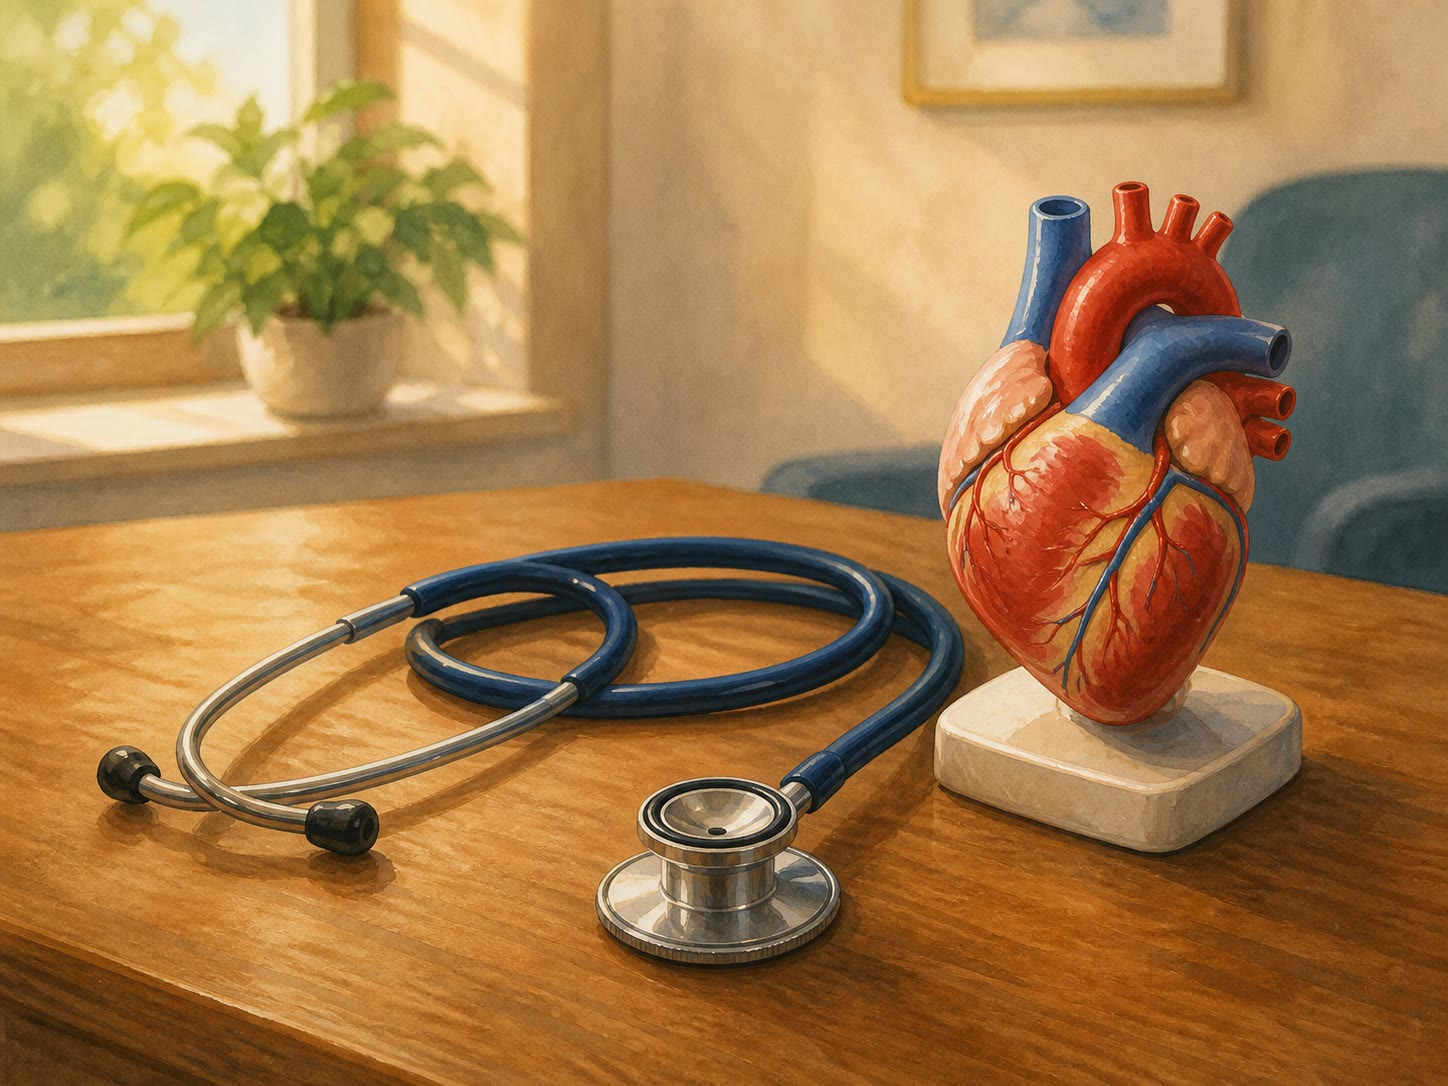
\includegraphics[width=0.56\linewidth]{images/book1/ai/g7-heart-stethoscope.jpg}

{\small 诊室中的两件经典器械：展示\omterm{def:g7:heart-and-circulation:rooms}{心室}和\omterm{def:g4:heart-and-blood:vessels}{血管}的模型，
以及能听出\omterm{def:g7:heart-and-circulation:rooms}{瓣膜}开闭之声的听诊器，
即听取\omterm{def:g7:heart-and-circulation:rooms}{瓣膜}关闭的声音。}
\end{omfigure}

\begin{proposition}[维护血管网络]\label{prop:g7:heart-and-circulation:keep}
\omterm{def:g4:heart-and-blood:vessels}{血管}网络的长期“敌人”与“朋友”已为人所知：
\begin{itemize}
  \item \emph{运动}能增强\omterm{def:g4:heart-and-blood:heart}{心脏}的泵力
        （\cref{prop:g7:organs-at-work:training}），并使
        \omterm{def:g4:heart-and-blood:vessels}{血管}保持柔韧；
  \item \emph{均衡饮食}
        （\cref{met:g3:balanced-diet:check}）能保护\omterm{def:g7:heart-and-circulation:vessels}{动脉}壁，
        防止\omterm{prop:g4:journey-of-food:absorb}{血液}中过多的脂质缓慢沉积，
        使其变厚、变硬；
  \item \emph{吸烟}既伤害肺，也伤害\omterm{def:g4:heart-and-blood:vessels}{血管}
        （\cref{prop:g7:lungs-and-gas-exchange:smoke}）——
        使\omterm{def:g4:heart-and-blood:vessels}{血管}变窄、变硬，挤占管腔；
  \item \omterm{def:g4:heart-and-blood:heart}{心脏}自身的供血——\omterm{def:g4:heart-and-blood:heart}{心脏}通过自己的小\omterm{def:g7:heart-and-circulation:vessels}{动脉}获取营养，
        而不是从心腔内的\omterm{prop:g4:journey-of-food:absorb}{血液}中获取——
        依赖于以上三者。
\end{itemize}
\cref{prop:g5:healthy-choices:contract}中的习惯，
实际上就是\omterm{def:g4:heart-and-blood:vessels}{血管}的日常维护。
\end{proposition}
\admitted

\begin{method}[将任一器官纳入血管网络]\label{met:g7:heart-and-circulation:map}
对本书涉及的任一器官：
\begin{enumerate}
  \item 将其置于体循环中：\omterm{def:g7:heart-and-circulation:vessels}{动脉}流入，\omterm{def:g7:heart-and-circulation:vessels}{静脉}流出，
        \omterm{def:g7:heart-and-circulation:vessels}{毛细血管}位于其中；
  \item 列出穿过其\omterm{def:g7:heart-and-circulation:vessels}{毛细血管}壁的物质进出情况
        （\omterm{prop:g7:digestion-and-nutrients:absorption}{绒毛}：吸收\omterm{def:g7:digestion-and-nutrients:families}{营养物质}；\omterm{def:g3:bones-and-muscles:muscle}{肌肉}：吸入燃料和
        \omterm{def:g7:what-is-respiration:respiration}{氧气}，排出\omterm{def:g7:what-is-respiration:respiration}{二氧化碳}；\omterm{def:g1:the-five-senses:sense}{皮肤}：散发热量）；
  \item 记下其特殊连接（如有）：\omterm{def:g4:journey-of-food:tract}{小肠}的\omterm{prop:g4:journey-of-food:absorb}{血液}
        先流经\omterm{prop:g7:digestion-and-nutrients:absorption}{肝脏}；肺则
        自成一个独立的循环。
  \item 对照器官的功能检查血流——
        \omterm{def:g4:heart-and-blood:vessels}{血管}网络图应能复述该器官
        的章节内容。
\end{enumerate}
\end{method}

\section{练习}

\begin{exercise}[$\star$]\label{exo:g7:heart-and-circulation:1}
说出\omterm{def:g4:heart-and-blood:heart}{心脏}的四个腔室，以及每个腔室的作用。
\end{exercise}

\begin{exercise}[$\star$]\label{exo:g7:heart-and-circulation:2}
\omterm{def:g4:heart-and-blood:heart}{心脏}\omterm{def:g7:heart-and-circulation:rooms}{瓣膜}的作用是什么，
“咚——哒”声又是什么？
\end{exercise}

\begin{exercise}[$\star$]\label{exo:g7:heart-and-circulation:3}
追踪两个循环，分别写出起点、终点和
回流路径。
\end{exercise}

\begin{exercise}[$\star$]\label{exo:g7:heart-and-circulation:4}
写出三类\omterm{def:g4:heart-and-blood:vessels}{血管}，
并分别说明一个结构特征和一种功能。
\end{exercise}

\begin{exercise}[$\star$]\label{exo:g7:heart-and-circulation:5}
为什么左\omterm{def:g7:heart-and-circulation:rooms}{心室}是壁最厚的腔室？
\end{exercise}

\begin{exercise}[$\star$]\label{exo:g7:heart-and-circulation:6}
全身所有的物质交换——在哪一类\omterm{def:g4:heart-and-blood:vessels}{血管}中发生——
呢？请列出三个器官的
\omterm{def:g7:heart-and-circulation:vessels}{毛细血管}交换。
\end{exercise}

\begin{exercise}[$\star\star$]\label{exo:g7:heart-and-circulation:7}
请以 \cref{ex:g7:heart-and-circulation:tour} 的路线，
追踪一滴为脑（而非大腿）供血的\omterm{prop:g4:journey-of-food:absorb}{血液}。
脑部\omterm{def:g7:heart-and-circulation:vessels}{毛细血管}的交换会取走什么、留下什么？
（\cref{prop:g5:brain-in-command:protect} 列出了脑
的需求。）
\end{exercise}

\begin{exercise}[$\star\star$]\label{exo:g7:heart-and-circulation:8}
\omterm{prop:g4:heart-and-blood:pulse}{脉搏}只在\omterm{def:g7:heart-and-circulation:vessels}{动脉}处能够触及，从不在\omterm{def:g7:heart-and-circulation:vessels}{静脉}处触及。
请结合两类\omterm{def:g4:heart-and-blood:vessels}{血管}的结构与压强作出解释。
\end{exercise}

\begin{exercise}[$\star\star$]\label{exo:g7:heart-and-circulation:9}
\omterm{def:g7:heart-and-circulation:vessels}{静脉}有单向\omterm{def:g7:heart-and-circulation:rooms}{瓣膜}，\omterm{def:g7:heart-and-circulation:vessels}{动脉}没有。\omterm{def:g7:heart-and-circulation:vessels}{静脉}\omterm{def:g7:heart-and-circulation:rooms}{瓣膜}
解决了什么问题——以及为什么站立不动的士兵
有时会晕倒？
\end{exercise}

\begin{exercise}[$\star\star$]\label{exo:g7:heart-and-circulation:10}
将 \cref{met:g7:heart-and-circulation:map} 用于
\omterm{def:g4:journey-of-food:tract}{小肠}，并包括其中的特殊连接。
\end{exercise}

\begin{exercise}[$\star\star$]\label{exo:g7:heart-and-circulation:11}
为什么\omterm{def:g4:heart-and-blood:heart}{心脏}需要自己的小供血\omterm{def:g7:heart-and-circulation:vessels}{动脉}，
其腔室中充满\omterm{prop:g4:journey-of-food:absorb}{血液}？而它们
的管壁增厚又为何如此重要？
\end{exercise}

\begin{exercise}[$\star\star\star$]\label{exo:g7:heart-and-circulation:12}
“\omterm{def:g4:heart-and-blood:heart}{心脏}是为\omterm{def:g7:heart-and-circulation:vessels}{毛细血管}服务的
管道。”请借助
\cref{rem:g7:heart-and-circulation:capillaries}，并
结合前面章节中的两种交换，为这一论断辩护。
\end{exercise}

\section{问题：心脏科医生的一个上午}

\begin{problem}[{周末问题——四次会诊，
一张网络图}]\label{pb:g7:heart-and-circulation:1}
跟随一位\omterm{def:g4:heart-and-blood:heart}{心脏}科医生度过一个上午，参与四场（虚构的）会诊，
手中持有网络图。

\medskip\noindent\textbf{第一部分——健康人的
基准。}
\begin{enumerate}
  \item 患者 1 是一名健康的青少年，她将接受
        路边测得的三项读数，见
        \cref{ex:g7:heart-and-circulation:measures}。
        请说出每项测量的名称，以及它测的是
        循环系统的哪一部分。
  \item 她的静息\omterm{prop:g4:heart-and-blood:pulse}{脉搏}为 $58$。\omterm{def:g4:heart-and-blood:heart}{心脏}科医生
        微笑。这是为什么
        （\cref{exo:g4:heart-and-blood:11}）？
  \item 她的心音清脆，呈双音。究竟是什么
        在每次心跳中两次猛然闭合？
  \item 画出她的\omterm{prop:g4:journey-of-food:absorb}{血液}自右\omterm{def:g7:heart-and-circulation:rooms}{心房}出发，绕行两条循环后返回的
        路径，以八个命名站点标示。
\end{enumerate}

\medskip\noindent\textbf{第二部分——三类问题。}
\begin{enumerate}[resume]
  \item 患者 2 的左\omterm{def:g7:heart-and-circulation:rooms}{心房}与左\omterm{def:g7:heart-and-circulation:rooms}{心室}之间\omterm{def:g7:heart-and-circulation:rooms}{瓣膜}漏，
        每次心跳都有部分\omterm{prop:g4:journey-of-food:absorb}{血液}向后倒流，
        并伴有呼啸样杂音。请预测这会如何影响
        体循环的输送，
        以及患者的耐力。
  \item 患者 3 是重度吸烟者，饮食丰富，
        \omterm{def:g7:heart-and-circulation:vessels}{动脉}增厚、变硬。
        会诊 1 中哪些读数会恶化，
        以及为何左\omterm{def:g7:heart-and-circulation:rooms}{心室}要超负荷工作？
  \item 患者 3 的\omterm{def:g7:heart-and-circulation:vessels}{动脉}增厚
        还包括\omterm{def:g4:heart-and-blood:heart}{心脏}自身的供血\omterm{def:g7:heart-and-circulation:vessels}{动脉}。
        请用一句话解释\omterm{def:g4:heart-and-blood:heart}{心脏}科医生的特别关切。
  \item 患者 4 长期站立后脚踝肿胀，
        \omterm{def:g7:heart-and-circulation:vessels}{静脉}的上行回流正在受阻。
        哪些结构正在失效，以及为何
        行走——小腿\omterm{def:g3:bones-and-muscles:muscle}{肌肉}挤压\omterm{def:g7:heart-and-circulation:vessels}{静脉}——
        能够缓解症状？
\end{enumerate}

\medskip\noindent\textbf{第三部分——挂图。}
\begin{enumerate}[resume]
  \item 诊所的挂图展示了双循环。
        请向候诊的患者解释，为何\omterm{prop:g4:journey-of-food:absorb}{血液}必须
        在每两次体循环之间都要流经肺。
  \item 补充\omterm{def:g4:heart-and-blood:vessels}{血管}图例：\omterm{def:g7:heart-and-circulation:vessels}{动脉}、\omterm{def:g7:heart-and-circulation:vessels}{毛细血管}、\omterm{def:g7:heart-and-circulation:vessels}{静脉}——
        各用一行说明其结构、压强与功能。
  \item 挂图的页脚写着：“所有治疗
        都服务于\omterm{def:g7:heart-and-circulation:vessels}{毛细血管}。”请以
        \cref{rem:g7:heart-and-circulation:capillaries} 为依据加以论证。
  \item 以\omterm{def:g4:heart-and-blood:heart}{心脏}科医生交给每位患者的
        预防处方结束这个上午：三条习惯，
        每条都与其机制相关，
        机制详见
        \cref{prop:g7:heart-and-circulation:keep}。
\end{enumerate}
\end{problem}
